%!TEX root = ../crowd_hierarchies_kdd.tex


\section{Experimental Evaluation}
\label{sec:exps}
We present an empirical evaluation of CRUX using both real and synthetic datasets. First, we discuss the experimental methodology, then we describe the data and results that demonstrate the effectiveness CRUX on crowdsourced entity extraction. The evaluation is performed on an Intel(R) Core(TM) i7 3.7 GHz 32GB machine; all algorithms are implemented in Python 2.7. 

\subsection{Experimental Setup}
\label{sec:expsetup}
\vspace{5pt}\noindent\textbf{Gain Estimators.} We evaluate the following gain estimators:
\squishlist
\item Chao92Shen: This estimator combines the methodology proposed by Chao~\cite{chao:1992} for estimating the number of unseen species  with Shen's formula, i.e., \Cref{eq:shen}.
\item HwangShen: This estimator combines the regression-based approach proposed by Hwang and Shen~\cite{hwang:2010} for estimating the number of unseen species $f_0$ with Shen's formula. 
\item NewRegr: This estimator corresponds to our new technique proposed in \Cref{sec:newestim}.
\squishend
All estimators are coupled with bootstrapping to estimate the gain variance used for retrieving an upper bound on the return of a query as shown in \Cref{sec:balancing}.

\vspace{5pt}\noindent\textbf{Entity Extraction Algorithms.} We evaluate the following algorithms for crowdsourced entity extraction:
\squishlist
\item Rand: This algorithm executes random queries until all the available budget is used. It selects a random node from the input poset $\hierarchy$ and a random query configuration $(k,l)$ from a list of pre-specified $k$, $l$ value combinations. \iftr We expect Rand to be effective for extracting entities in small and dense data domains that do not have many sparsely populated nodes. \fi
\item RandL: Same as Rand but only executes queries {\em only at the lowest level nodes} (i.e., leaf nodes) of the input poset $\hierarchy$ until all the available budget is used.  \iftr We expect RandL to be effective for {\em shallow} data domains when the majority of nodes corresponds to leaf nodes. Like Rand, the performance of RandL is expected to be reasonable for small and dense data domains without sparsely populated nodes.\fi
\item BFS: This algorithm performs a breadth-first traversal of the input poset $\hierarchy$, executing one query at each node. The query configuration is randomly selected from a list of pre-specified $k$, $l$ value combinations. This algorithm promotes exploration of the action space when extracting entities. \iftr It also takes into account the structure of the input domain but is agnostic to sparsely populated nodes of the input $\hierarchy$. \fi
\item RootChao: This algorithm corresponds to the entity extraction scheme of Trushkowsky et al.~\cite{trushkowsky:2013} that utilizes the Chao92Shen estimator to measure the gain of an additional query. The proposed scheme is agnostic to the structure of the input entity domain, and thus, equivalent to issuing queries only at the root node of the poset $\hierarchy$. Since the authors only propose a pay-as-you-go scheme, we coupled this algorithm with Alg.~\ref{algo:overall} to optimize for the input budget constraint. We allowed the algorithm to consider different query configurations $(k,l)$ but restricted the possible queries to the root node.
\item GSChao, GSWang, GSNewR: We try different variations of CRUX. These algorithms correspond to our proposed graph search querying policy algorithm (\Cref{sec:heuristic}) coupled with Chao92Shen, HwangShen and NewRegr respectively.
\item GSExact: This algorithm is used as a near-optimal, omniscient baseline that allows us to see how far off our algorithms are from an algorithm with perfect information. We combine the algorithm proposed in \Cref{sec:heuristic} with an exact computation of the return or gains from queries. The algorithm proceeds as follows: At each round we speculatively execute each of the available actions (i.e., all query configurations across all nodes) and select the one that results in the largest number of return to cost ratio. Since the return of each query is known, the algorithm is not coupled with any of the aforementioned estimators.
\squishend

Rand, RandL and BFS promote the exploration of the action space when extracting entities, while the other algorithms balance exploration with exploitation. For the results reported below, we run each algorithm ten times and report the average gain achieved under the given budget.

\vspace{5pt}\noindent\textbf{Querying Interface.} For all datasets we consider generalized queries $q^v(k,E)$. The nodes $v$ are set based on the input poset and $(k,l)$ takes values in {\small $\{(5,0), (10,0), (20,0)$, $(5,2), (10,5), (20,5), (20,10)\}$}. Larger values of $k$ or $l$ were deemed unreasonable for crowdsourced queries. The gain of a query is computed as the number of new entities extracted. The cost of each query is computed using an additive model comprised by three partial cost terms that depend on the characteristics of the query. 

The three partial cost terms are: (i) {\sf CostK} that depends on the number of responses $k$ requested from a user, (ii) {\sf CostL} that depends on the size of the exclude list $l$ used in the query, and (iii) {\sf CostSpec} that depends on the {\em specificity} of the query $q_s$, e.g., we assume that queries that require users to provide more specialized entities (e.g., ``list one concert for New York on the 17th of Nov'') cost more than more generic queries (e.g.,  ``list one concert in New York''). More formally, we define the specificity of a query to be equal to the number of attributes assigned non-wildcard values for the node $u \in \hierarchy$ the query corresponds to. 

We consider two types of cost functions. The first one corresponds to a linear function where the overall cost for a query with configuration $(k,l)$ with specificity $s$ is computed as:{\scriptsize $Cost(q) = \alpha \cdot \frac{k}{\mbox{max. query size}} + \beta \cdot  \frac{l}{\mbox{max. ex. list size}} + \gamma \cdot  \frac{s}{\mbox{max. specificity}} $}. The cost of a query should be significantly increased when an exclude list is used, thus $\beta$ should be set to a larger value than $\alpha$ and $\gamma$. Different $(\alpha, \beta, \gamma)$ configurations were tested. We also considered a step cost function ${\sf CostK} + {\sf CostL}$, where {\sf CostK} and {\sf CostL} are set as follows: $(k,{\sf CostK} = \{(5,\$0.20), (10,\$0.60), (20,\$0.80)\}$ and $(l,{\sf CostL} = \{(0,\$0), (2,\$0.10), (5,\$0.50), (10,\$0.70)\}$. We observed that the {\em relative performance} of the extraction algorithms for different cost functions was the similar. In the discussion below, we report the cost function we used for each experiment. 

\vspace{5pt}\noindent\textbf{Data.} First, we evaluate the proposed framework on extracting entities from a large sparse domain. We consider a dataset extracted from Eventbrite (see\Cref{sec:intro}). We collected a dataset spanning over 63 countries that are divided into 1,709 subareas (e.g., states) and 10,739 cities, containing events of 19 different types, such as rallies, tournaments, conferences, conventions, etc. and a time period of 31 days spanning over the months of October and November. The dataset is described by three dimensions: (i) event type, (ii) location, and (iii) time. Two of the three dimensions, i.e., location and time, are hierarchically structured. The poset characterizing the domain can be fully specified if we consider the cross product across the possible values for location, event type and time. For each of the location, time, type dimensions we also consider a special {\em wildcard} value. Taking the cross-product across the possible values of these dimensions results in poset with a total of 8,508,160 nodes containing 57,805 distinct events overall. We point out that only 175,068 nodes are populated leading to a rather sparsely populated domain. Due to lack of popularity proxies for the extracted events, we assigned a random {\em popularity value} in $(0,10]$ to each event. These weights are used to form the actual popularity distribution characterizing the population of each node in the poset. 

We further evaluate the performance of the extraction algorithms for a more dense domain, that we constructed ourselves. As described in ~\Cref{sec:intro}, we used Amazon's Mechanical Turk (AMT)~\cite{mturk} to collect a real-world dataset, targeted at extracting ``people in the news''. This domain is still structured and the attributes characterizing it are the occupation of each person and the news portal. We asked workers to extract the names of people belonging to four different occupations from five different news portals. The people occupations we considered are ``Politicians'', ``Athletes'', ``Actors/Singers'' and ``Industry People''. The news portals we considered are ``New York Times'', ``Huffington Post'', ``Washington Post'', ``USA  Today'' and ``The Wall Street Journal''. 

This data domain, referred to as the PeopleInNews, is essentially characterized by the type of the individual and the news portal. Workers were paid \$0.20 per HIT. We issued 20 HITS for each leaf node of the domain's poset, resulting in 600 HITS in total. After manually curating name misspelling's, we extracted 1,245 unique people in total. The popularity value of each extracted entity was assigned to be equal to the number of distinct workers that reported it. The values are normalized during to form a proper popularity distribution. Collecting a large amount of data in advance from A and then simulating the responses of human workers by revealing portions of this dataset allows us to compare different algorithms on an equal footing; this approach is often adopted in the evaluation of crowdsourcing algorithms~\cite{DBLP:journals/pvldb/ParameswaranBG0PW14, marcus:2011,trushkowsky:2013}.

%\begin{table}
%\center
%\caption{The population characteristics for PeopleInNews.}
%\label{tab:ptypedata}
%\begin{tabular}{|c|c|}
%\hline
%\textbf{Occupation} & \textbf{People} \\ \hline
%Industry People & 743 \\
%Athletes & 743 \\
%Politicians & 748 \\
%Actors/Singers & 744 \\ \hline
%\end{tabular}
%\quad
%\begin{tabular}{|c|c|}
%\hline
%\textbf{News Portal} & \textbf{People} \\ \hline
%WSJ & 594 \\
%WashPost & 597 \\
%NY Times & 595 \\
%HuffPost & 599 \\
%USA Today & 593 \\ \hline
%\end{tabular}
%\vspace{-10pt}
%\end{table}

\subsection{Experimental Results}
We evaluate different aspects of the above extraction techniques. The results reported in Figures 4-8 correspond to a linear cost function with $\alpha=\gamma=1$ and $\beta=5$. The results in Figure 9 correspond to the step cost function described above.

\vspace{3pt}\noindent{\textbf{How does CRUX compare against baselines?}}
We evaluate the performance of the different extraction algorithms in terms of number of entities extracted for different budgets. The results for Eventbrite and PeopleInNews are shown in \Cref{fig:ebextraction} and \Cref{fig:poextraction} respectively. As shown, CRUX, i.e., GSChao, GSHwang, GSNewR {\em outperform all baselines for at least 30\% across both datasets}. This behavior is expected as our techniques not only exploit the structure of the domain to diversify entity extraction by targeting entities that belong to the tail of the popularity distribution but also optimize the queries for the given budget.

When comparing again the naive baselines Rand, RandL, and BFS, we see that GSChao, GSHwang and GSNewR extract at least 2X more entities for the sparse Eventbrite domain and around 100\% more entities for small budgets and 54\% for larger ones when considering the dense PeopleInNews. For example for Eventibrite and a budget of \$50 all schemes coupled with our querying policy discovery algorithm (\Cref{sec:solving}) extracted more than 600 events while Rand and RandL extracted 1.1 and 0.2 events and BFS extracted 207.7 events, an improvement of over 180\%.

Comparing against RootChao, we see that GSChao, GSHwang and GSNewR, are able to retrieve up to 30\% more entities for Eventbrite and 5X for the PeopleInNews. This performance difference is due to the fact that the gain achieved by RootChao saturates at a faster rate compared to GSChao, GSHwang and GSNewR as the cost increases. This is because, RootChao focuses on issuing queries at the root of the input poset, and hence, it is not able to extract entities belonging to the long tail of the popularity distribution. Moreover, for the PeopleInNews we see that RootChao performs poorly even compared to the naive baselines Rand, RandL and BFS. Again, this behavior is due to the skew of the underlying popularity distribution.

\begin{figure}[h]
\begin{center}
        \subfigure{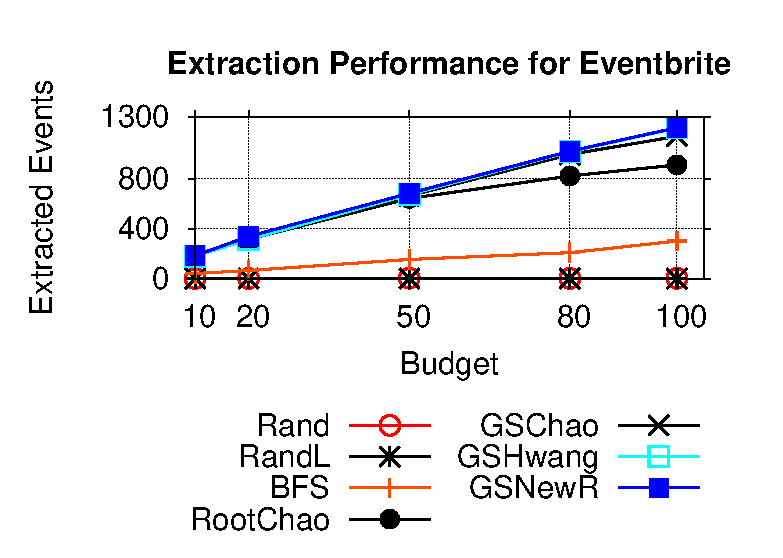
\includegraphics[trim=120 0 0 0,scale=0.40]{figs/ebExtractionNotOpt.eps} \label{fig:ebextraction}}
        \subfigure{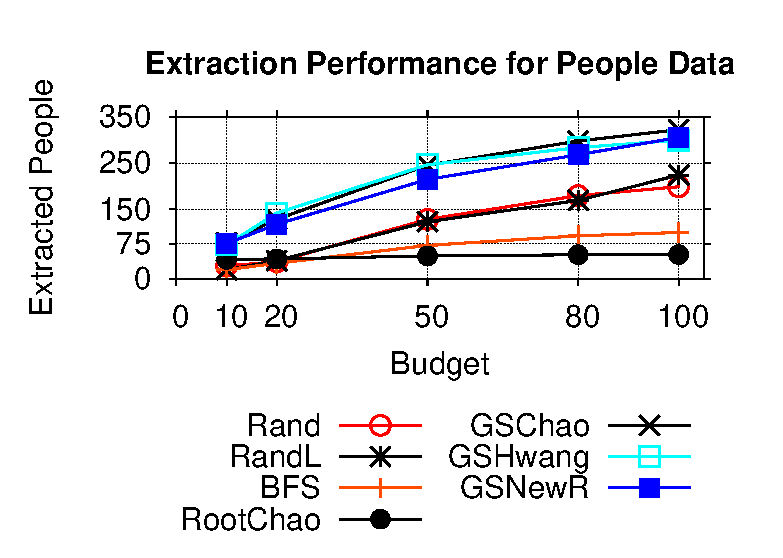
\includegraphics[trim=80 0 100 0,scale=0.40]{figs/poExtractionNotOpt.eps} \label{fig:poextraction}}
        \subfigure{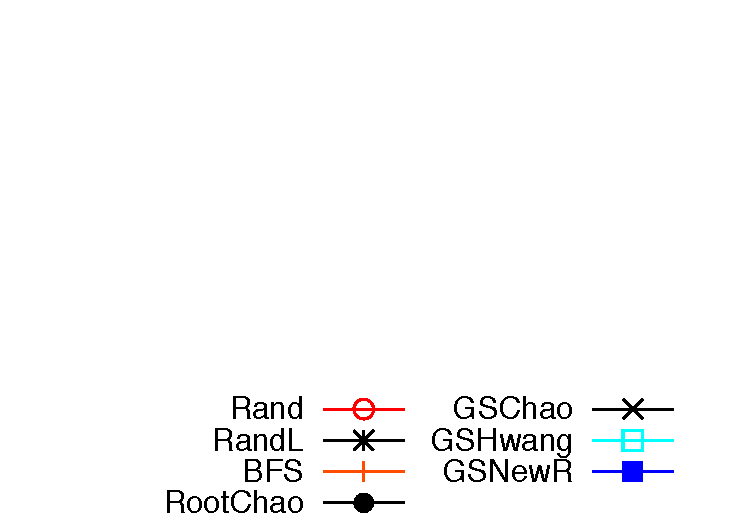
\includegraphics[scale=0.30]{figs/notoptlegend.pdf}}
\end{center}
\vspace{-5pt}
\caption{A comparison of the CRUX techniques (GSChao, GSHwang, and GSNewR) against baselines for (a) Eventbrite and (b) PeopleInNews.}
\label{fig:resultsextr}
\vspace{-10pt}
\end{figure}

\vspace{3pt}\noindent{\textbf{How does CRUX compare against a near-optimal policy discovery algorithm?}}
Next, we evaluate the different variations of CRUX, i.e., GSChao, GSHwang and GSNewR, against the near-optimal querying policy discovery algorithm GSExact. The results for Eventbrite and PeopleInNews are shown in \Cref{fig:ebextractionopt} and \Cref{fig:poextractionopt} respectively. Regarding the dense domain Eventbrite, we observe that for smaller budgets our proposed techniques perform comparably to GSExact that has ``perfect information'' about the gain of each query, typically demonstrating a performance gap of less than 10\%. For larger budgets this gap increases to 25\%. Note that our estimators have access to few samples and sparse information; the fact that we are able to get this close to GSExact is notable. Finally, for PeopleInNews, our techniques present an increased performance gap compared to GSExact. Nevertheless the performance drop is at most 50\%. 

\begin{figure}[h]
\begin{center}
        \subfigure{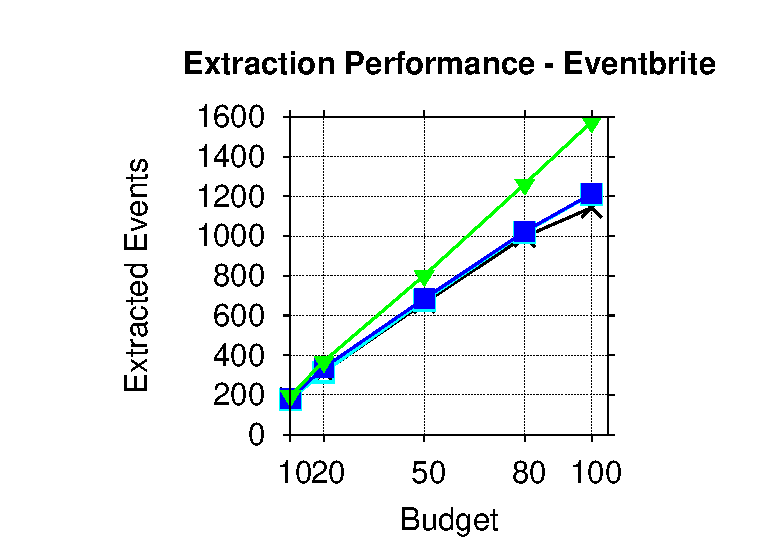
\includegraphics[trim=120 0 0 0,scale=0.40]{figs/ebExtractionOpt.eps} \label{fig:ebextractionopt}}
        \subfigure{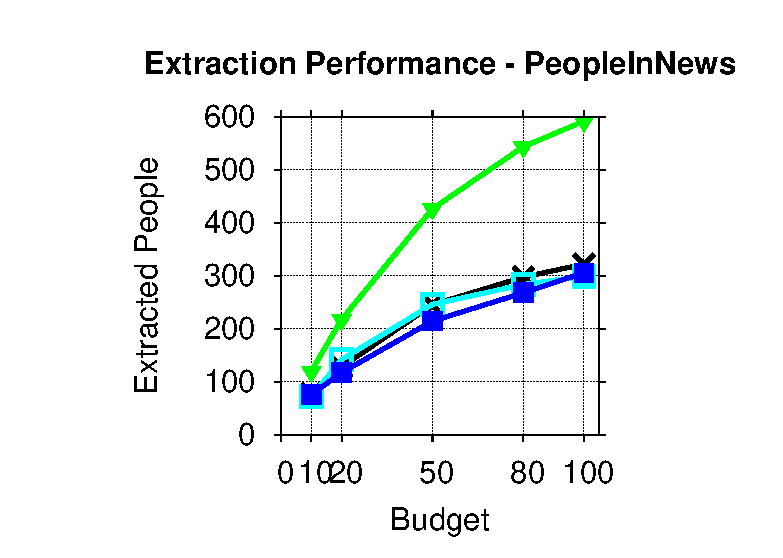
\includegraphics[trim=80 0 100 0,scale=0.40]{figs/poExtractionOpt.eps} \label{fig:poextractionopt}}
        \subfigure{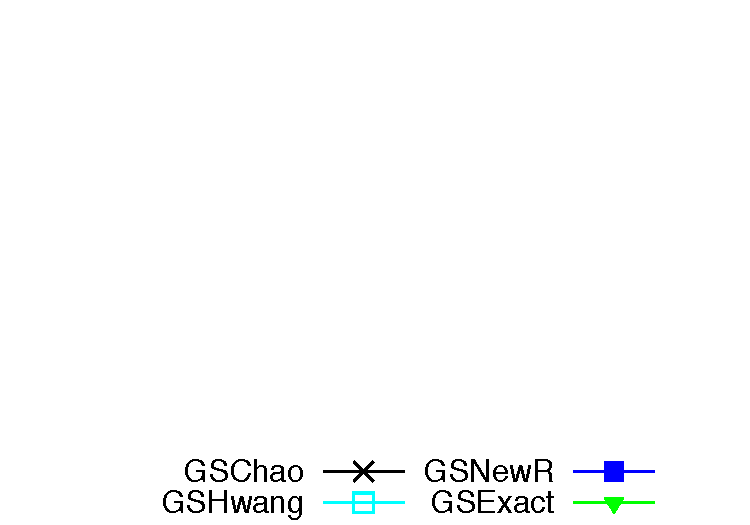
\includegraphics[scale=0.30]{figs/optlegend.pdf}}
\end{center}
\vspace{-5pt}
\caption{A comparison of the CRUX techniques (GSChao, GSHwang, and GSNewR) against a near-optimal algorithm for (a) Eventbrite and (b) PeopleInNews.}
\label{fig:resultsextr}
\vspace{-10pt}
\end{figure}

\vspace{3pt}\noindent{\textbf{How do the different techniques compare with respect to the total number of queries issued during extraction?}}
We compare the performance of RootChao (i.e., the extraction scheme proposed by Trushkowsky et al.~\cite{trushkowsky:2013}) against the CRUX algorithms GSChao, GSHwang and GSNewR with respect to the {\em total number of queries issued during extraction}. Notice that this new evaluation metric characterizes directly the overall latency of the crowd-extraction process. \Cref{fig:rounds} shows the corresponding results for a run for Eventbrite and a budget of \$80. As shown {\em RootChao requires almost up to 3x more queries} to extract the same number of entities as our proposed techniques, thus, exhibiting significantly larger latency compared to GSChao, GSHwang and GSNewR.

\begin{figure}[h]
	\begin{center}
	\vspace{-10pt}
	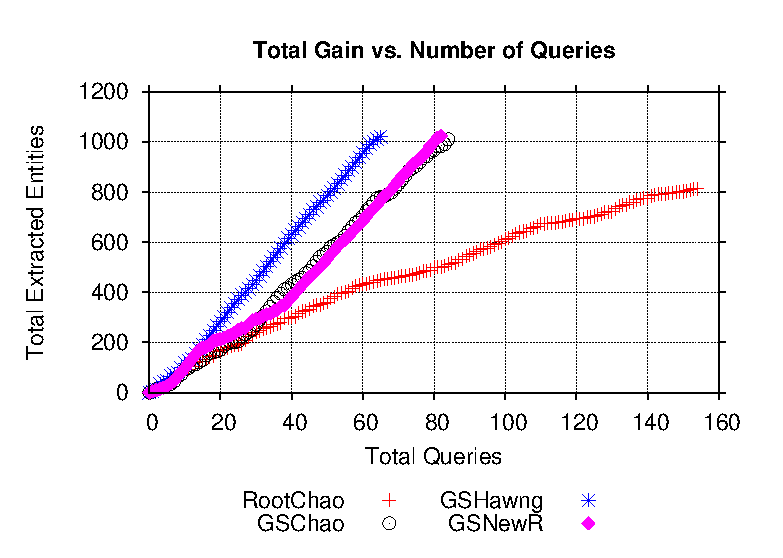
\includegraphics[clip,scale=0.5]{figs/gain_rounds.eps}
	\caption{The number of events extracted by different algorithms for Eventbrite versus the total number of queries.}
	\label{fig:rounds}
	\end{center}
	\vspace{-20pt}
\end{figure}

\vspace{3pt}\noindent{\textbf{How do our different algorithms traverse the poset and use different query configurations?}}
We next explore how the different versions of CRUX traverse the poset, and how they use different query configurations. The results reported are averaged over ten runs and correspond to PeopleInNews. We begin by considering how many queries these algorithms issue at various levels of the poset. In Figure~\ref{fig:level}, we plot the different number of queries issued at various levels by our algorithms when the budget is set to 10 and 100 respectively. Given a small budget, we observe that all algorithms prefer issuing queries at higher levels of the poset. Notice that inner nodes of the poset are preferred and only a small number of queries is issued at the root (i.e., level one) of the poset. This behavior is justified if we consider that due to their popularity, certain entities are repeatedly extracted, thus leading to a lower gain. As the budget increases, we see that all algorithms tend to consider more specialized queries at deeper levels of the poset. It is interesting to observe that all of our algorithms issue the majority of their queries at the level two nodes, while GSExact, which has perfect information, focuses mostly on the leaf nodes. Thus, in this case, our techniques could benefit from being more aggressive at traversing the poset and reaching deeper levels; overall, our techniques may end up being more conservative in order to cater to a larger space of posets and popularity distributions. In Figure~\ref{fig:queryconf}, we plot the different query configurations chosen by our algorithms when the budget is set to 10 and 100 respectively. We observe that GSExact always prefers queries with $k = 20$ and $l = 0$ for both small and large budgets. On the other hand, our algorithms issue more queries of smaller size when operating under a limited budget and prefer queries of larger size for larger budgets. Out of all algorithms we see that GSNewR was the only one issuing queries with exclude lists of different sizes, thus exploiting the rich diversity of query interfaces. However, the number of such queries is limited. 


\begin{figure}[h]
    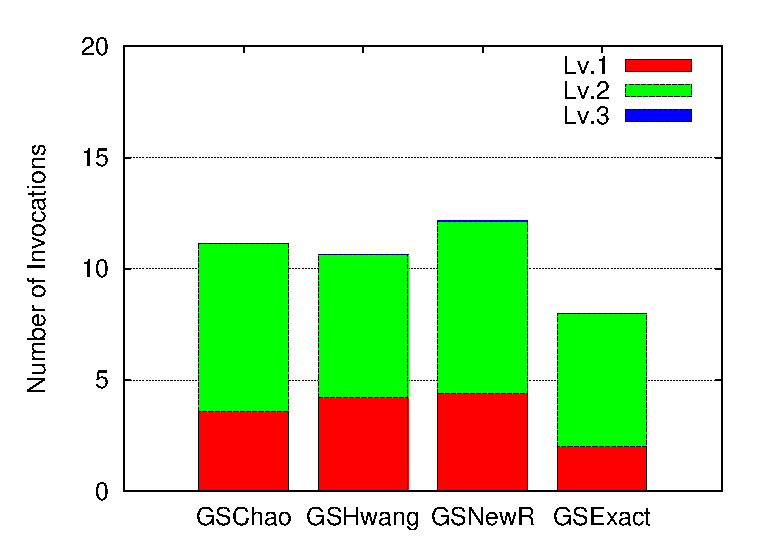
\includegraphics[clip,scale=0.32]{figs/levelBudget10.eps}
	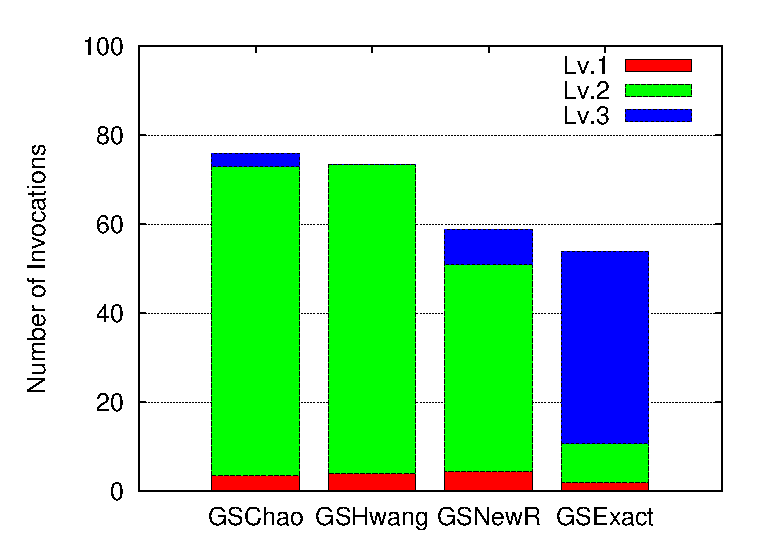
\includegraphics[clip,scale=0.32]{figs/levelBudget100.eps}
	\caption{The number of queries issued at different levels used when budget is set at 10 or 100.}\label{fig:level}
\end{figure}

\begin{figure}[h]
   	 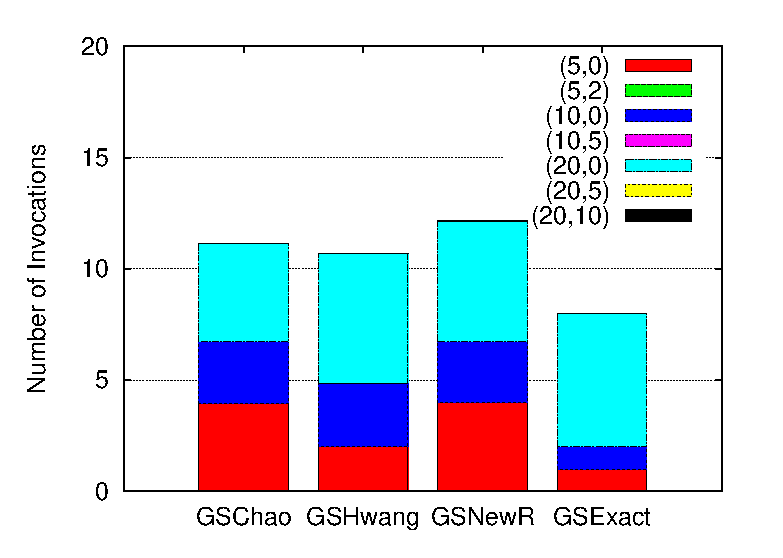
\includegraphics[clip,scale=0.32]{figs/queryConfBudget10.eps}
	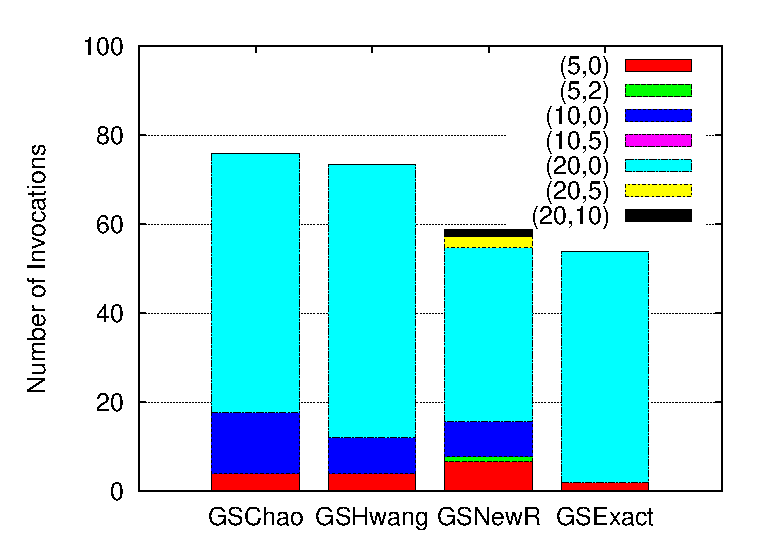
\includegraphics[clip,scale=0.32]{figs/queryConfBudget100.eps}
	\caption{The query configurations used when budget is set at 10 or 100.}\label{fig:queryconf}
		\vspace{-20pt}
\end{figure}

\vspace{3pt}\noindent{\textbf{Are exclude lists helpful?}} In \Cref{fig:queryconf} we see that only GSNewR made use of exclude lists. However, we observed a drastically different behavior when using a step cost function. \Cref{fig:exEffect} shows the performance of GSChao with and without the use of exclude lists and compares that with the performance of GSExact that uses exclude lists. The results correspond to PeopleInNews. We see that exploiting exclude lists can yield performance improvements up to 50\% especially for larger budgets.

\begin{figure}[h]
	\begin{center}
	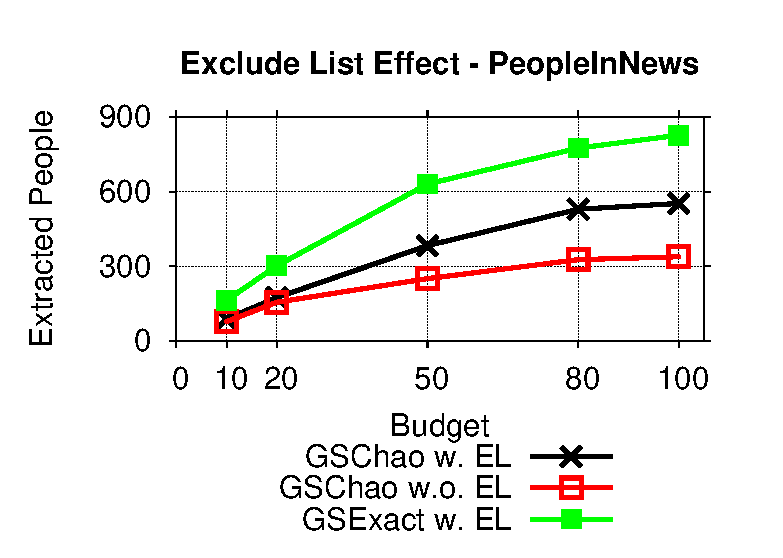
\includegraphics[clip,scale=0.5]{figs/exEffect.eps}
	\caption{Using an exclude list under a step cost function provides significant extraction gains.}
	\label{fig:exEffect}
	\end{center}
	\vspace{-20pt}
\end{figure}

\vspace{3pt}\noindent{\textbf{How effective are the different estimators at predicting the gain of additional queries?}}
Finally, we point out that GSNewR was able to outperform GSChao and GSHwang for Eventbrite but the opposite behavior was observed for the PeopleInNews. To further understand the relative performance of GSChao, GSHwang and GSNewR, we evaluate the performance of the gain estimators Chao92Shen, HwangShen and NewRegr at predicting the number of new retrieved events for different query configurations. For Eventbrite, we choose ten random nodes containing more than 5,000 events and for each of them and each of the available query parameter configurations $(k,l)$, we execute ten queries of the form ``Give me $k$ items from node $u \in \hierarchy$ that are not included in an exclude list of size $l$''. As mentioned in \Cref{sec:excludelist} the exclude list for each query is constructed following a randomized approach.  For PeopleInNews, we issue ten queries over all nodes of the input poset for all available query configurations.  We measure the performance of each estimator by considering the absolute relative error between the predicted return and the actual return of the query. 

\begin{table}[h]
\scriptsize \center
\vspace{-10pt}
\caption{Average absolute relative error for estimating the gain of different queries for Eventbrite.}
\label{tab:eventesterror}
\begin{tabular}{|c|c|c|c|c|}
\hline
\textbf{Q. Size $k$} & \textbf{EL. Size $l$} & \textbf{Chao92Shen} & \textbf{HwangShen} & \textbf{NewRegr} \\ \hline
5 & 0 & 0.470 & 0.500 & 0.390 \\
5 & 2 & 0.554 & 0.612 & 0.467\\
10 & 0 & 0.569 & 0.592 & 0.544\\
10 & 5 & 0.580 & 0.696 & 0.29\\
20 & 0 & 0.642 & 0.756 &0.471\\
20 & 5 & 0.510 & 0.60 & 0.436 \\
20 & 10 & 0.653 & 0.756 & 0.631\\
\hline
\end{tabular}
\end{table}


\Cref{tab:eventesterror} reports the relative error for each of the three estimators averaged over all points under consideration for Eventbrite. As shown, all three estimators perform equivalently with the new regression-based technique slightly outperforming Chao92Shen and HwangShen for certain types of queries. For example, for $k = 10, l = 5$, Chao92Shen has a relative error of 0.58, HwangShen had a relative error of 0.7, and NewRegr had a relative error of 0.29. We attribute the improved extraction performance of GSNewR to these improved estimates. The relatively large values for relative errors are justified as the retrieved samples correspond to a very small portion of the underlying population for each of the points. This is a well-known behavior for non-parametric estimators and studied extensively in the species estimation literature~\cite{hwang:2010}. 

\begin{table}[h]
\scriptsize \center
\caption{Average absolute percentage error for estimating the gain of different queries for PeopleInNews.}
\label{tab:peopleesterror}
\begin{tabular}{|c|c|c|c|c|}
\hline
\textbf{Q. Size $k$} & \textbf{EL. Size $l$} & \textbf{Chao92Shen} & \textbf{HwangShen} & \textbf{NewRegr} \\ \hline
5 & 0 & 0.295 & 0.299 & 0.228\\
5 & 2 & 0.163 &  0.156 & 0.144\\
10 & 0 &  0.306 & 0.305 & 0.277\\
10 & 5 &  0.341 & 0.349 & 0.293\\
20 & 0 &  0.359& 0.371 & 0.467 \\
20 & 5 &  0.2615 & 0.264 & 0.249\\
20 & 10 & 0.1721 & 0.162 & 0.127\\
\hline
\end{tabular}
\end{table}

\Cref{tab:peopleesterror} shows the results for PeopleInNews. We observe that for smaller query sizes the regression technique proposed in this paper offers better gain estimates. However, as the query size increases, and hence, a larger portion of the underlying population is observed Chao92Shen outperforms both regression-based techniques. Thus, we are able to explain the performance difference between GSChao and the other two algorithms. Eventually, we have that for sparse domains regression-based techniques result in better performance. However, for dense domains the Chao92Shen estimator results in better performance as a larger portion of the underlying population can be sampled. 




